\documentclass{article}\usepackage[]{graphicx}\usepackage[]{color}
%% maxwidth is the original width if it is less than linewidth
%% otherwise use linewidth (to make sure the graphics do not exceed the margin)
\makeatletter
\def\maxwidth{ %
  \ifdim\Gin@nat@width>\linewidth
    \linewidth
  \else
    \Gin@nat@width
  \fi
}
\makeatother

\definecolor{fgcolor}{rgb}{0.345, 0.345, 0.345}
\newcommand{\hlnum}[1]{\textcolor[rgb]{0.686,0.059,0.569}{#1}}%
\newcommand{\hlstr}[1]{\textcolor[rgb]{0.192,0.494,0.8}{#1}}%
\newcommand{\hlcom}[1]{\textcolor[rgb]{0.678,0.584,0.686}{\textit{#1}}}%
\newcommand{\hlopt}[1]{\textcolor[rgb]{0,0,0}{#1}}%
\newcommand{\hlstd}[1]{\textcolor[rgb]{0.345,0.345,0.345}{#1}}%
\newcommand{\hlkwa}[1]{\textcolor[rgb]{0.161,0.373,0.58}{\textbf{#1}}}%
\newcommand{\hlkwb}[1]{\textcolor[rgb]{0.69,0.353,0.396}{#1}}%
\newcommand{\hlkwc}[1]{\textcolor[rgb]{0.333,0.667,0.333}{#1}}%
\newcommand{\hlkwd}[1]{\textcolor[rgb]{0.737,0.353,0.396}{\textbf{#1}}}%

\usepackage{framed}
\makeatletter
\newenvironment{kframe}{%
 \def\at@end@of@kframe{}%
 \ifinner\ifhmode%
  \def\at@end@of@kframe{\end{minipage}}%
  \begin{minipage}{\columnwidth}%
 \fi\fi%
 \def\FrameCommand##1{\hskip\@totalleftmargin \hskip-\fboxsep
 \colorbox{shadecolor}{##1}\hskip-\fboxsep
     % There is no \\@totalrightmargin, so:
     \hskip-\linewidth \hskip-\@totalleftmargin \hskip\columnwidth}%
 \MakeFramed {\advance\hsize-\width
   \@totalleftmargin\z@ \linewidth\hsize
   \@setminipage}}%
 {\par\unskip\endMakeFramed%
 \at@end@of@kframe}
\makeatother

\definecolor{shadecolor}{rgb}{.97, .97, .97}
\definecolor{messagecolor}{rgb}{0, 0, 0}
\definecolor{warningcolor}{rgb}{1, 0, 1}
\definecolor{errorcolor}{rgb}{1, 0, 0}
\newenvironment{knitrout}{}{} % an empty environment to be redefined in TeX

\usepackage{alltt}

\usepackage{amsmath}
\usepackage{Rd}
\usepackage{verbatim}

\usepackage[round]{natbib}
\bibliographystyle{abbrvnat}

%\VignetteIndexEntry{Black-Scholes-Merton and the Greeks}
%\VignetteDepends{GARPFRM}
%\VignettePackage{GARPFRM}
\IfFileExists{upquote.sty}{\usepackage{upquote}}{}

\begin{document}





\title{Black-Scholes-Merton and the Greeks}
\author{Ross Bennett}

\maketitle

\begin{abstract}
The purpose of this vignette is to demonstrate the Black-Scholes-Merton pricing formulas and the "Greeks" as outlined in Chapter 4 and Chapter 5 of Valuation and Risk Models.
\end{abstract}

\tableofcontents

\section{Black-Scholes-Merton Pricing Formulas}
This section focuses on the application of the Black-Scholes-Merton pricing formulas for European call and put options. For derivation and theoretical background, the reader is encouraged to to study Chapter 4 of Valuation and Risk Models.

The Black-Scholes-Merton pricing formulas for European call and put options are
\begin{description}
  \item[Call]
  \begin{equation*}
  c = S_0 N(d_1) - K e^{-rT} N(d_2)
  \end{equation*}
  \item[Put]
  \begin{equation*}
  p = K e^{-rT} N(-d_2) - S_0 N(-d_1)
  \end{equation*}
\end{description}

where
\begin{eqnarray*}
  d_1 = \frac{\ln (S_0 / K) + (r + \sigma^2 / 2) T}{\sigma \sqrt{T}}\\
  d_2 = \frac{\ln (S_0 / K) + (r - \sigma^2 / 2) T}{\sigma \sqrt{T}} = d_1 - \sigma \sqrt{T}\\
  S_0 \quad \text{is the underlying stock price at $t = 0$}\\
  K \quad \text{is the strike price}\\
  r \quad \text{is the risk free rate}\\
  T \quad \text{is the time to maturity in years}\\
  \sigma \quad \text{is the volatility of the stock}\\
  N(.) \quad \text{is the cumulative distribution function for a standard normal distribution}
\end{eqnarray*}

\subsection{Properties}
For a call option, as the underlying price, $S_0$, becomes very large, the option will almost surely be exercised. The price of the call then becomes

\begin{equation*}
S_0 - K e^{-r T}
\end{equation*}

\begin{knitrout}
\definecolor{shadecolor}{rgb}{0.969, 0.969, 0.969}\color{fgcolor}\begin{kframe}
\begin{alltt}
\hlcom{# Demonstrate the property of the Black-Scholes-Merton formula for a call }
\hlcom{# option as the underlying price becomes very large}
S0 <- \hlkwd{seq}(100, 100000, 100)
eu.call <- \hlkwd{optionSpec}(style = \hlstr{"european"}, 
                      type = \hlstr{"call"}, 
                      S0 = S0,
                      K = 100,
                      maturity = 1, 
                      r = 0.1, 
                      volatility = 0.2)
call.price <- \hlkwd{optionValue}(option = eu.call, method = \hlstr{"Black-Scholes"})
\hlkwd{plot}(S0, call.price, xlab=\hlstr{"Underlying Price"}, ylab=\hlstr{"Call Price"},
     main=\hlstr{"Call price as S_0 becomes very large"}, type=\hlstr{"l"})
\end{alltt}
\end{kframe}
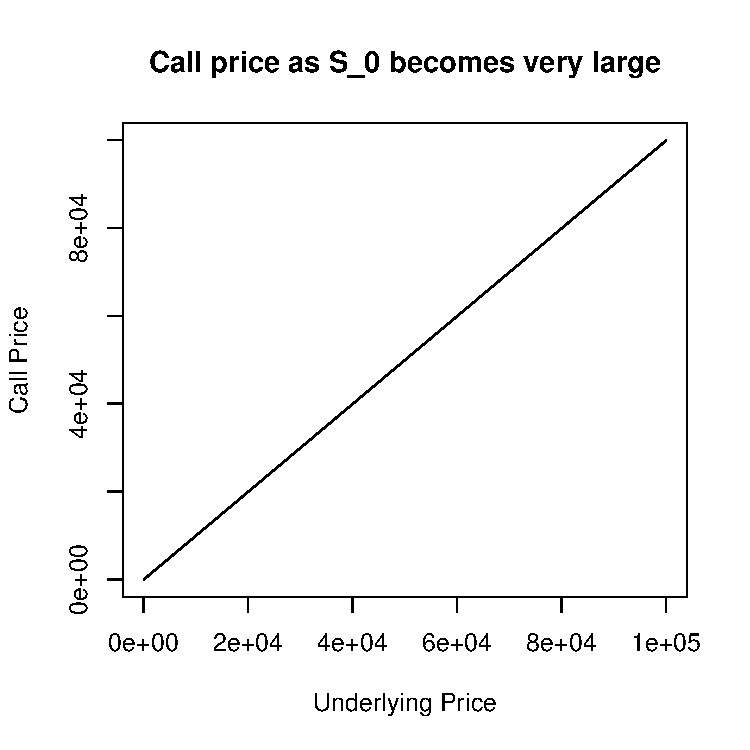
\includegraphics[width=\maxwidth]{figure/unnamed-chunk-2} 

\end{knitrout}


\begin{knitrout}
\definecolor{shadecolor}{rgb}{0.969, 0.969, 0.969}\color{fgcolor}\begin{kframe}
\begin{alltt}
\hlcom{# Demonstrate the property of the Black-Scholes-Merton formula for a call }
\hlcom{# option as the volatility approaches 0}
sigma <- \hlkwd{seq}(0.2, 0, -0.01)
eu.call <- \hlkwd{optionSpec}(style = \hlstr{"european"}, 
                      type = \hlstr{"call"}, 
                      S0 = 100,
                      K = 100,
                      maturity = 1, 
                      r = 0.1, 
                      volatility = sigma)
call <- \hlkwd{optionValue}(option = eu.call, method = \hlstr{"Black-Scholes"})
\hlcom{# S_0 - K * e^\{-r T\}}
100 - 100 * \hlkwd{exp}(-0.1 * 1)
\end{alltt}
\begin{verbatim}
## [1] 9.516
\end{verbatim}
\begin{alltt}
\hlkwd{plot}(sigma, call, ylab=\hlstr{"Call Price"}, xlab=\hlstr{"Volatility"}, 
     main=\hlstr{"Call price as volatility approaches 0"}, type = \hlstr{"l"})
\end{alltt}
\end{kframe}
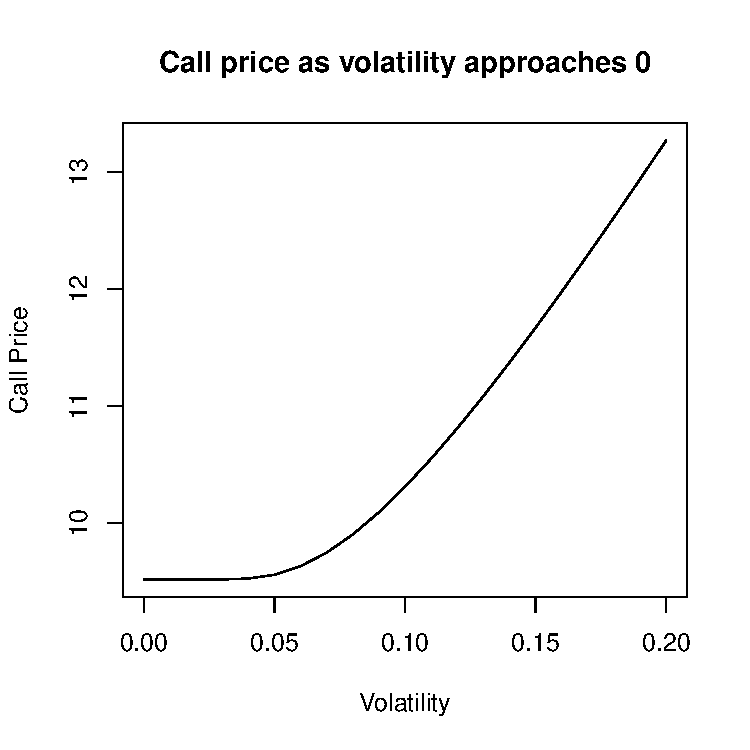
\includegraphics[width=\maxwidth]{figure/unnamed-chunk-3} 

\end{knitrout}



Example 4.6: The stock price 6 months for the expiration of an option is \$42, the exercise price of the option is \$40, the risk-free interest rate is 10\% per annum, and the volatility is 20\% per annum.
\begin{knitrout}
\definecolor{shadecolor}{rgb}{0.969, 0.969, 0.969}\color{fgcolor}\begin{kframe}
\begin{alltt}
\hlcom{# The stock price 6 months for the expiration of an option is $42, }
\hlcom{# the exercise price of the option is $40, the risk-free interest }
\hlcom{# rate is 10% per annum, and the volatility is 20% per annum.}

\hlcom{# Price the European call option}
eu.call <- \hlkwd{optionSpec}(style = \hlstr{"european"}, 
                      type = \hlstr{"call"}, 
                      S0 = 42, 
                      K = 40,
                      maturity = 0.5, 
                      r = 0.1, 
                      volatility = 0.2)
call <- \hlkwd{optionValue}(option = eu.call, method = \hlstr{"Black-Scholes"})
call
\end{alltt}
\begin{verbatim}
## [1] 4.759
\end{verbatim}
\begin{alltt}

\hlcom{# Price the European put option}
eu.put <- eu.call
eu.put$type <- \hlstr{"put"}
put <- \hlkwd{optionValue}(option = eu.put, method = \hlstr{"Black-Scholes"})
put
\end{alltt}
\begin{verbatim}
## [1] 0.8086
\end{verbatim}
\end{kframe}
\end{knitrout}


\section{Implied Volatilities}
The volatility the stock price is not directly observable and must be implied by option prices in the market. Here we calculate the implied volatility of a European call option with a price of \$1.875 and $S_0 = 21$, $K = 20$, $r = 0.1$, and $T = 0.25$. 
\begin{knitrout}
\definecolor{shadecolor}{rgb}{0.969, 0.969, 0.969}\color{fgcolor}\begin{kframe}
\begin{alltt}
\hlcom{# Compute the implied volatility of a European call option with a }
\hlcom{# price of $1.875 and S_0 = 21, K = 20, r = 0.1, and T = 0.25}
eu.call <- \hlkwd{optionSpec}(style = \hlstr{"european"}, 
                      type = \hlstr{"call"}, 
                      S0 = 21, 
                      K = 20,
                      maturity = 0.25, 
                      r = 0.1)
\hlkwd{impliedVolatility}(eu.call, 1.875)
\end{alltt}
\begin{verbatim}
## [1] 0.2345
\end{verbatim}
\end{kframe}
\end{knitrout}


\section{Dividends}
Example 4.9: Consider a European call option on a stock when there are ex-dividend dates in two months and five months. The dividend on each ex-dividend date is expected to be \$0.50. The current share price is \$40, the exercise price is \$40, and the stock price volatility is 30\% per annum, the risk-free rate of interest is 9\% per annum, and the time to maturity is 6 months. 
Here we compute the value of a European call option with known dividends. 
\begin{knitrout}
\definecolor{shadecolor}{rgb}{0.969, 0.969, 0.969}\color{fgcolor}\begin{kframe}
\begin{alltt}
\hlcom{# Consider a European call option on a stock when there are }
\hlcom{# ex-dividend dates in two months and five months. The dividend }
\hlcom{# on each ex-dividend date is expected to be \textbackslash{}$0.50. The current }
\hlcom{# share price is \textbackslash{}$40, the exercise price is \textbackslash{}$40, and the stock }
\hlcom{# price volatility is 30\textbackslash{}% per annum, the risk-free rate of }
\hlcom{# interest is 9\textbackslash{}% per annum, and the time to maturity is 6 months.}

\hlcom{# Subtract the present value of the dividends from the underlying price}
S0 <- 40 - (0.5 * \hlkwd{exp}(-0.09 * 2 / 12) + 0.5 * \hlkwd{exp}(-0.09 * 5 / 12))
eu.call <- \hlkwd{optionSpec}(style = \hlstr{"european"}, 
                      type = \hlstr{"call"}, 
                      S0 = S0, 
                      K = 40,
                      maturity = 0.5, 
                      r = 0.09,
                      volatility = 0.3)
\hlkwd{optionValue}(eu.call, \hlstr{"Black-Scholes"})
\end{alltt}
\begin{verbatim}
## [1] 3.671
\end{verbatim}
\end{kframe}
\end{knitrout}



\section{The Greek Letters}
This section introduces what is referred to as the "Greeks" for European options using the Black-Scholes-Merton formulas. The Greeks measure risk in a position in an option or portfolio of options.

Here we create option specifications for call and put options that will be used in the following sections.
\begin{knitrout}
\definecolor{shadecolor}{rgb}{0.969, 0.969, 0.969}\color{fgcolor}\begin{kframe}
\begin{alltt}
\hlcom{# Specify European call and put options where the current stock price is}
\hlcom{# $49, the strike price is $50, the risk-free rate is 5%, the time to}
\hlcom{# maturity is 20 weeks, and the volatility is 20%.}

eu.call <- \hlkwd{optionSpec}(style = \hlstr{"european"}, 
                      type = \hlstr{"call"}, 
                      S0 = 49, 
                      K = 50,
                      maturity = 20/52, 
                      r = 0.05,
                      volatility = 0.2)

eu.put <- \hlkwd{optionSpec}(style = \hlstr{"european"}, 
                      type = \hlstr{"put"}, 
                      S0 = 49, 
                      K = 50,
                      maturity = 20/52, 
                      r = 0.05,
                     volatility = 0.2)
\end{alltt}
\end{kframe}
\end{knitrout}



\subsection{Delta}
The delta ($\Delta$) of an option is defined as the rate of change of the option price with respect to the price of te underlying asset.

The delta of a European option is given as
\begin{eqnarray*}
\Delta (call) = N(d_1)\\
\Delta (put) = N(d_1) - 1\\
\end{eqnarray*}

\begin{knitrout}
\definecolor{shadecolor}{rgb}{0.969, 0.969, 0.969}\color{fgcolor}\begin{kframe}
\begin{alltt}
\hlcom{# Compute the delta of the European call option}
\hlkwd{computeGreeks}(eu.call, \hlstr{"delta"})
\end{alltt}
\begin{verbatim}
## [1] 0.5216
\end{verbatim}
\end{kframe}
\end{knitrout}



\begin{knitrout}
\definecolor{shadecolor}{rgb}{0.969, 0.969, 0.969}\color{fgcolor}\begin{kframe}
\begin{alltt}
\hlcom{# Delta as the underlying price varies}
\hlkwd{computeGreeks}(eu.call, \hlstr{"delta"}, prices = \hlkwd{seq}(20, 80, 1), 
              plot = TRUE, main=\hlstr{"Delta of call"})
\end{alltt}
\end{kframe}
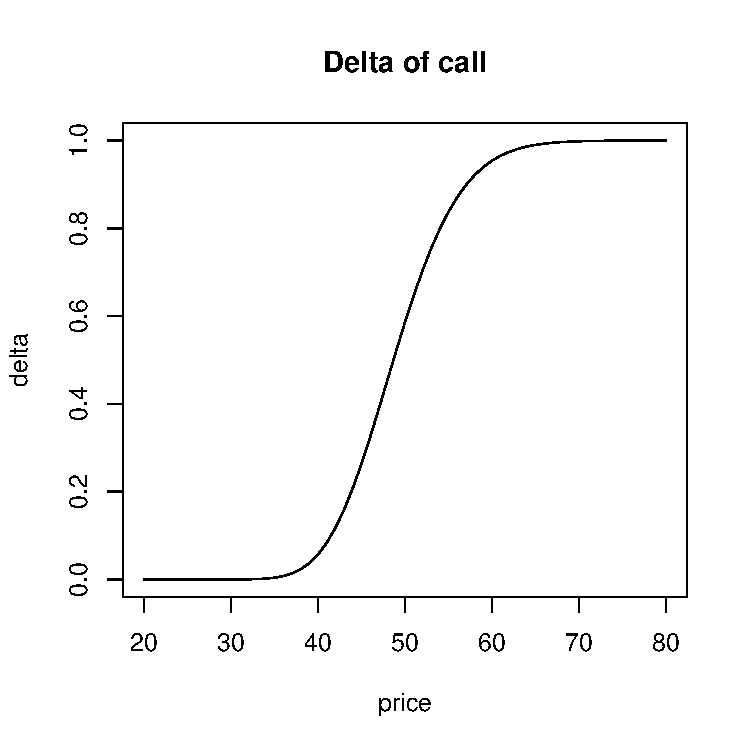
\includegraphics[width=\maxwidth]{figure/unnamed-chunk-91} 
\begin{kframe}\begin{alltt}
\hlkwd{computeGreeks}(eu.put, \hlstr{"delta"}, prices = \hlkwd{seq}(20, 80, 1), 
              plot = TRUE, main=\hlstr{"Delta of put"})
\end{alltt}
\end{kframe}
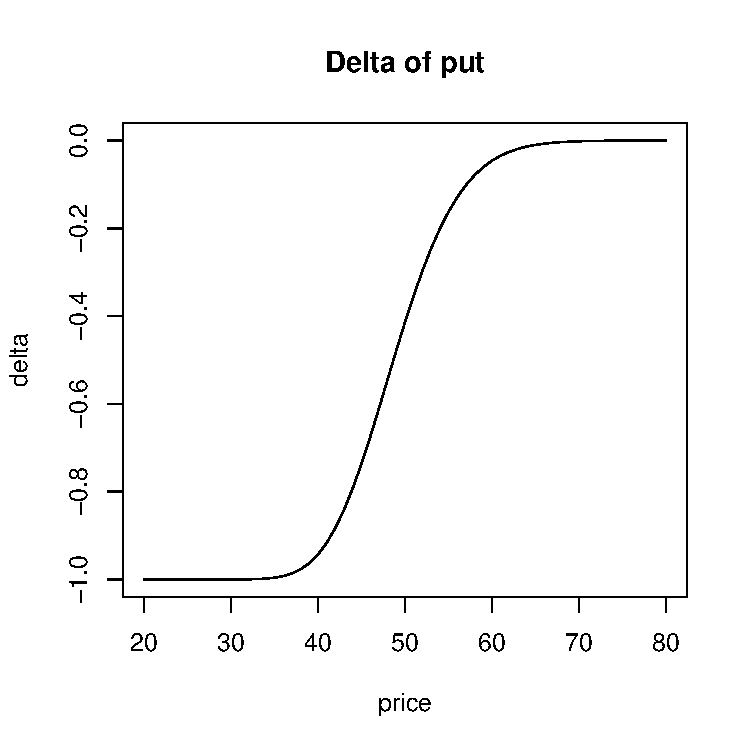
\includegraphics[width=\maxwidth]{figure/unnamed-chunk-92} 

\end{knitrout}


\begin{knitrout}
\definecolor{shadecolor}{rgb}{0.969, 0.969, 0.969}\color{fgcolor}\begin{kframe}
\begin{alltt}
\hlcom{# Delta as the time to maturity varies for in the money, at the money, and}
\hlcom{# out of the money call options}
maturity <- \hlkwd{seq}(0.01, 1, 0.05)
\hlkwd{plot}(maturity, xlim = \hlkwd{range}(maturity), ylim = \hlkwd{c}(0,1), 
     type=\hlstr{"n"}, xlab=\hlstr{"Time to expiration"}, ylab=\hlstr{"Delta"})
\hlkwd{lines}(x = maturity, y = \hlkwd{deltaBS}(52, 50, 0.05, 0, 0.2, maturity, \hlstr{"call"}), 
      lty=2, col=\hlstr{"blue"})
\hlkwd{lines}(x = maturity, y = \hlkwd{deltaBS}(50, 50, 0.05, 0, 0.2, maturity, \hlstr{"call"}), 
      lty=1, col=\hlstr{"black"})
\hlkwd{lines}(x = maturity, y = \hlkwd{deltaBS}(48, 50, 0.05, 0, 0.2, maturity, \hlstr{"call"}), 
      lty=3, col=\hlstr{"red"})
\hlkwd{title}(\hlstr{"Delta of call"})
\hlkwd{legend}(\hlstr{"topright"}, legend=\hlkwd{c}(\hlstr{"In the money"}, \hlstr{"At the money"}, \hlstr{"Out of the money"}),
       lty=\hlkwd{c}(2,1,3), col=\hlkwd{c}(\hlstr{"blue"}, \hlstr{"black"}, \hlstr{"red"}), bty=\hlstr{"n"}, cex=0.8)
\end{alltt}
\end{kframe}
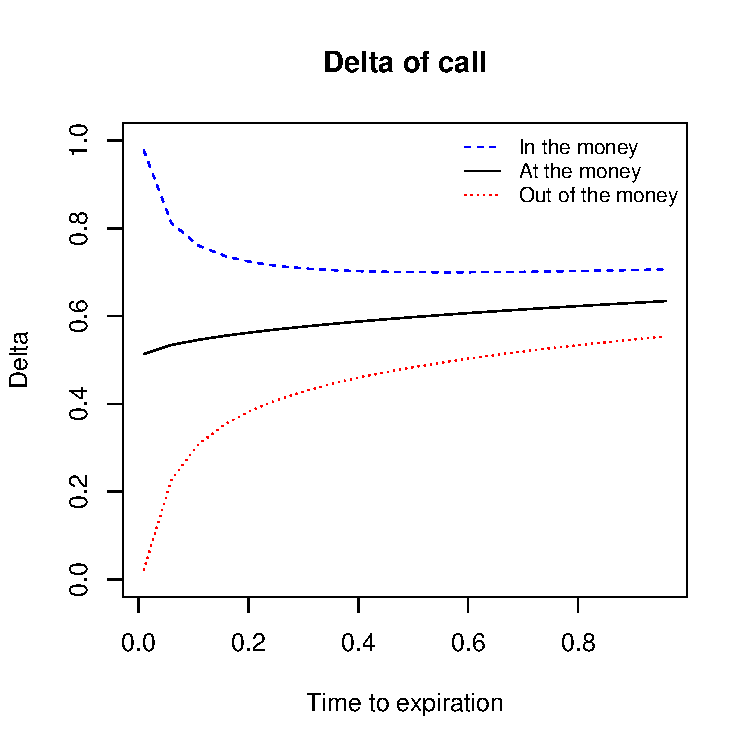
\includegraphics[width=\maxwidth]{figure/unnamed-chunk-10} 

\end{knitrout}


The delta of a portfolio of options is simply the sum of the delta's of the individual options.

\begin{equation*}
\Delta_P = \sum_{i=1}^n w_i \Delta_i
\end{equation*}

Suppose a financial instituion has the following three positions in options on a stock.
\begin{enumerate}
  \item A long position in 100,000 call options with the strike price of \$55 and an expiration date in 3 months. The delta of each option is 0.533.
  \item A short position in 200,000 call options with stick price of \$56 and an expiration date in 2 months. The delta of each option is 0.468.
  \item A short position in 50,000 options with strike price of \$56 and an expiration date in 2 months. The delta of each option is -0.508.
\end{enumerate}

The delta of the portfolio is
\begin{knitrout}
\definecolor{shadecolor}{rgb}{0.969, 0.969, 0.969}\color{fgcolor}\begin{kframe}
\begin{alltt}
100000 * 0.533 - 200000 * 0.468 - 50000 * -0.508
\end{alltt}
\begin{verbatim}
## [1] -14900
\end{verbatim}
\end{kframe}
\end{knitrout}


This means that the portfolio can be made delta neutral by purchasing 14,900 shares of the underlying stock.


\subsection{Theta}
The theta ($\Theta$) of an option is defined as the rate of change of the value of the option with respect to the passage of time with all else remaining equal.

The theta of a European option is given as
\begin{eqnarray*}
\Theta (call) = - \frac{S_0 N'(d_1) \sigma}{2 \sqrt{T}} - r K e^{-r T} N(d_2)\\
\Theta (put) = \frac{S_0 N'(d_1) \sigma}{2 \sqrt{T}} + r K e^{-r T} N(-d_2)\\
\end{eqnarray*}

where $N'(.)$ is the probability density function for a standard normal distribution.

\begin{knitrout}
\definecolor{shadecolor}{rgb}{0.969, 0.969, 0.969}\color{fgcolor}\begin{kframe}
\begin{alltt}
\hlcom{# Compute the theta of the European call option}
\hlkwd{computeGreeks}(eu.call, \hlstr{"theta"})
\end{alltt}
\begin{verbatim}
## [1] -4.305
\end{verbatim}
\end{kframe}
\end{knitrout}


\begin{knitrout}
\definecolor{shadecolor}{rgb}{0.969, 0.969, 0.969}\color{fgcolor}\begin{kframe}
\begin{alltt}
\hlcom{# Theta as the underlying price varies}
\hlkwd{computeGreeks}(eu.call, \hlstr{"theta"}, prices = \hlkwd{seq}(20, 80, 1), 
              plot = TRUE, main=\hlstr{"Theta of call"})
\end{alltt}
\end{kframe}
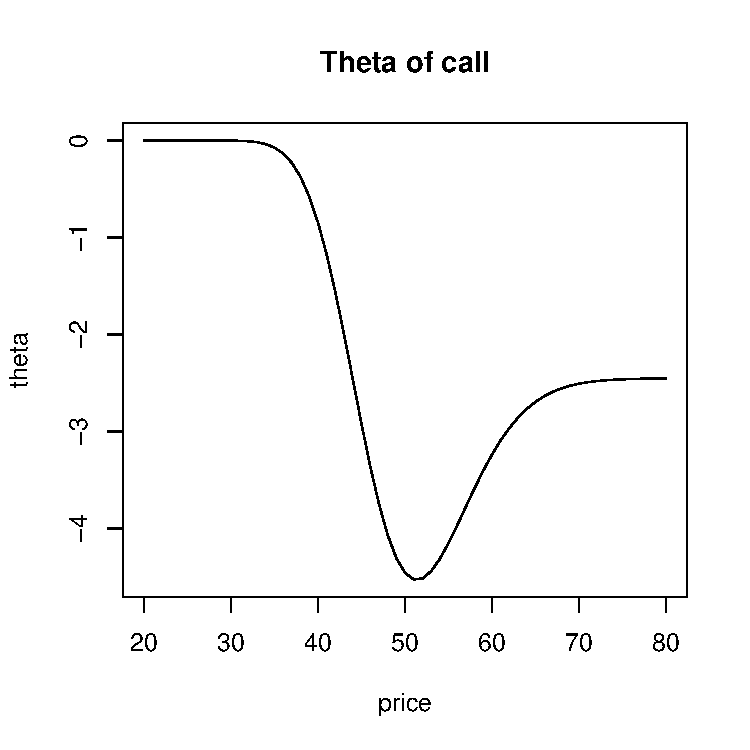
\includegraphics[width=\maxwidth]{figure/unnamed-chunk-13} 

\end{knitrout}


\begin{knitrout}
\definecolor{shadecolor}{rgb}{0.969, 0.969, 0.969}\color{fgcolor}\begin{kframe}
\begin{alltt}
\hlcom{# Theta as the time to maturity varies for in the money, at the money, and}
\hlcom{# out of the money call options}
maturity <- \hlkwd{seq}(0.01, 1, 0.05)
\hlkwd{plot}(maturity, xlim = \hlkwd{range}(maturity), ylim = \hlkwd{c}(-15,0), 
     type=\hlstr{"n"}, xlab=\hlstr{"Time to expiration"}, ylab=\hlstr{"Theta"})
\hlkwd{lines}(x = maturity, y = \hlkwd{thetaBS}(55, 50, 0.05, 0, 0.2, maturity, \hlstr{"call"}), 
      lty=2, col=\hlstr{"blue"})
\hlkwd{lines}(x = maturity, y = \hlkwd{thetaBS}(50, 50, 0.05, 0, 0.2, maturity, \hlstr{"call"}), 
      lty=1, col=\hlstr{"black"})
\hlkwd{lines}(x = maturity, y = \hlkwd{thetaBS}(45, 50, 0.05, 0, 0.2, maturity, \hlstr{"call"}), 
      lty=3, col=\hlstr{"red"})
\hlkwd{title}(\hlstr{"Theta of call"})
\hlkwd{legend}(\hlstr{"topright"}, legend=\hlkwd{c}(\hlstr{"In the money"}, \hlstr{"At the money"}, \hlstr{"Out of the money"}),
       lty=\hlkwd{c}(2,1,3), col=\hlkwd{c}(\hlstr{"blue"}, \hlstr{"black"}, \hlstr{"red"}), bty=\hlstr{"n"}, cex=0.8)
\end{alltt}
\end{kframe}
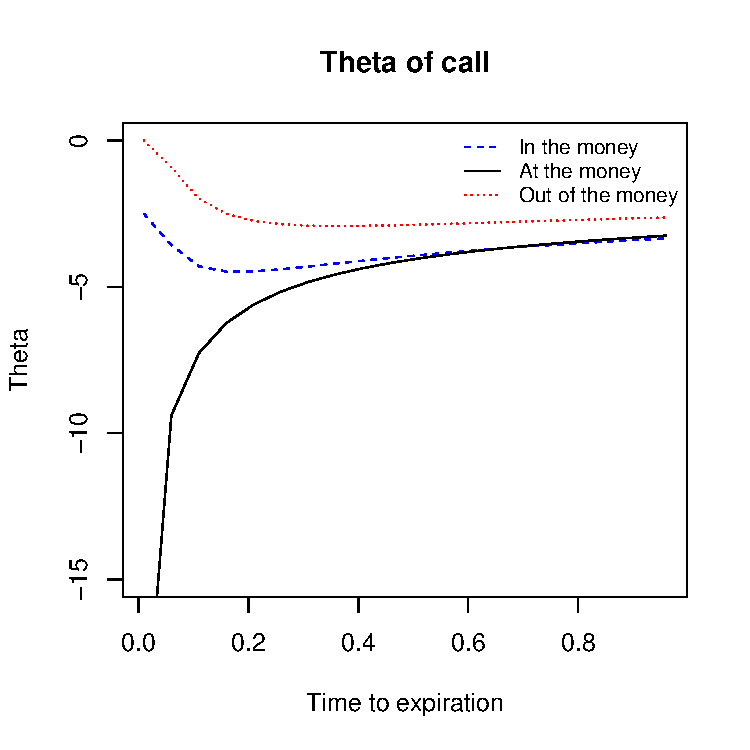
\includegraphics[width=\maxwidth]{figure/unnamed-chunk-14} 

\end{knitrout}


\subsection{Gamma}
The gamma ($\Gamma$) of an option is defined as the rate of change of the delta of the option with respect to the price of the underlying asset.

The gamma of a European option is given as
\begin{equation*}
\Gamma = \frac{N'(d_1)}{S_0 \sigma \sqrt{T}}
\end{equation*}

Note that the gamma for a European put option is equal to the gamma of a European call option.

\begin{knitrout}
\definecolor{shadecolor}{rgb}{0.969, 0.969, 0.969}\color{fgcolor}\begin{kframe}
\begin{alltt}
\hlcom{# Compute the gamma of the European call option}
\hlkwd{computeGreeks}(eu.call, \hlstr{"gamma"})
\end{alltt}
\begin{verbatim}
## [1] 0.06554
\end{verbatim}
\end{kframe}
\end{knitrout}


\begin{knitrout}
\definecolor{shadecolor}{rgb}{0.969, 0.969, 0.969}\color{fgcolor}\begin{kframe}
\begin{alltt}
\hlcom{# Gamma as the underlying price varies}
\hlkwd{computeGreeks}(eu.call, \hlstr{"gamma"}, prices = \hlkwd{seq}(20, 80, 1), 
              plot = TRUE, main=\hlstr{"Gamma of call"})
\end{alltt}
\end{kframe}
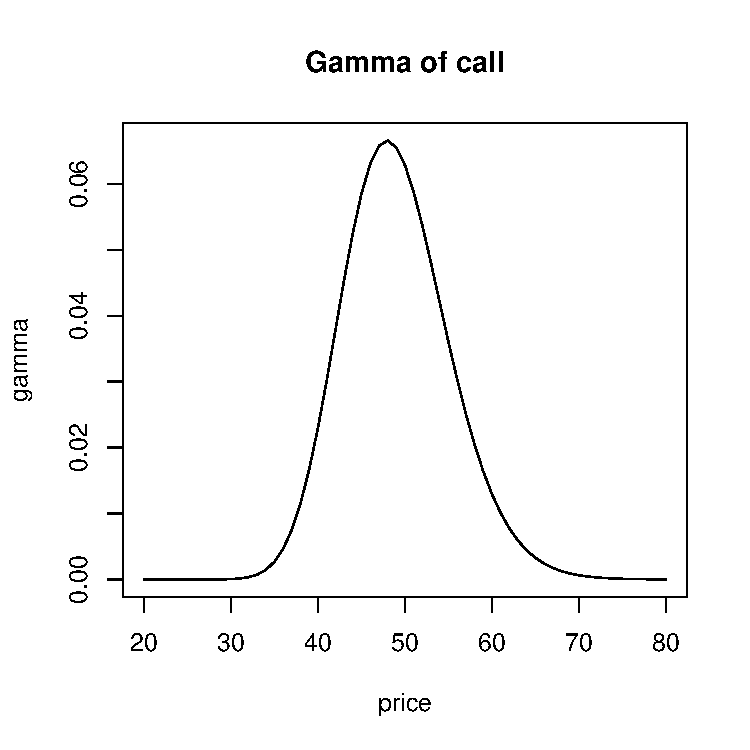
\includegraphics[width=\maxwidth]{figure/unnamed-chunk-16} 

\end{knitrout}


\begin{knitrout}
\definecolor{shadecolor}{rgb}{0.969, 0.969, 0.969}\color{fgcolor}\begin{kframe}
\begin{alltt}
\hlcom{# Gamma as the time to maturity varies for in the money, at the money, and}
\hlcom{# out of the money call options}
maturity <- \hlkwd{seq}(0.01, 1, 0.05)
\hlkwd{plot}(maturity, xlim = \hlkwd{range}(maturity), ylim = \hlkwd{c}(0,0.5), 
     type=\hlstr{"n"}, xlab=\hlstr{"Time to expiration"}, ylab=\hlstr{"Gamma"})
\hlkwd{lines}(x = maturity, y = \hlkwd{gammaBS}(55, 50, 0.05, 0, 0.2, maturity, \hlstr{"call"}), 
      lty=2, col=\hlstr{"blue"})
\hlkwd{lines}(x = maturity, y = \hlkwd{gammaBS}(50, 50, 0.05, 0, 0.2, maturity, \hlstr{"call"}), 
      lty=1, col=\hlstr{"black"})
\hlkwd{lines}(x = maturity, y = \hlkwd{gammaBS}(45, 50, 0.05, 0, 0.2, maturity, \hlstr{"call"}), 
      lty=3, col=\hlstr{"red"})
\hlkwd{title}(\hlstr{"Gamma of call"})
\hlkwd{legend}(\hlstr{"topright"}, legend=\hlkwd{c}(\hlstr{"In the money"}, \hlstr{"At the money"}, \hlstr{"Out of the money"}),
       lty=\hlkwd{c}(2,1,3), col=\hlkwd{c}(\hlstr{"blue"}, \hlstr{"black"}, \hlstr{"red"}), bty=\hlstr{"n"}, cex=0.8)
\end{alltt}
\end{kframe}
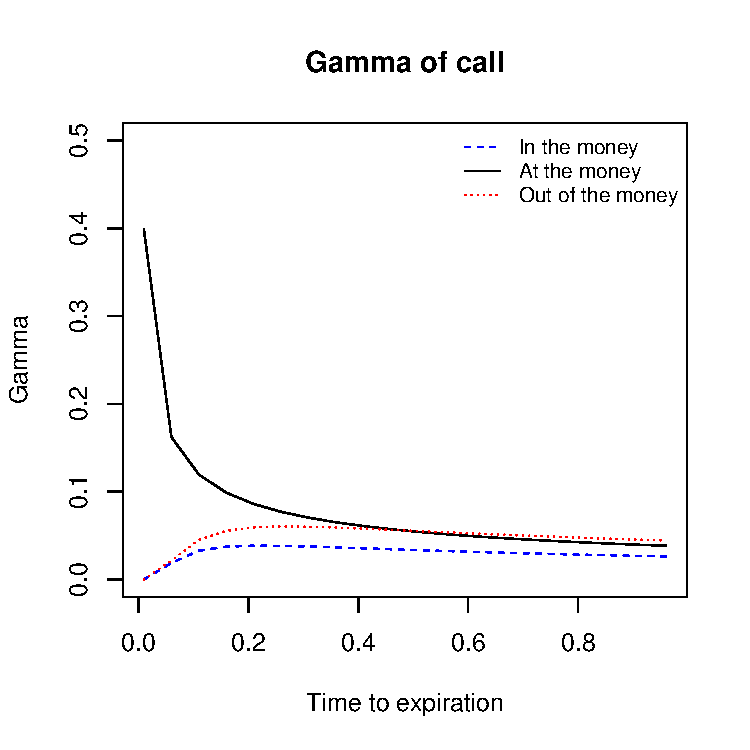
\includegraphics[width=\maxwidth]{figure/unnamed-chunk-17} 

\end{knitrout}


\subsection{Vega}
The vega ($\nu$) of an option is defined as the rate of change of the value of the option with respect to the volatility of the underlying asset.

The vega of a European option is given as
\begin{equation*}
\nu = S_0 \sqrt{T} N'(d_1)
\end{equation*}

Note that the vega for a European put option is equal to the vega of a European call option.

\begin{knitrout}
\definecolor{shadecolor}{rgb}{0.969, 0.969, 0.969}\color{fgcolor}\begin{kframe}
\begin{alltt}
\hlcom{# Compute the vega of a European call option}
\hlkwd{computeGreeks}(eu.call, \hlstr{"vega"})
\end{alltt}
\begin{verbatim}
## [1] 12.11
\end{verbatim}
\end{kframe}
\end{knitrout}


\begin{knitrout}
\definecolor{shadecolor}{rgb}{0.969, 0.969, 0.969}\color{fgcolor}\begin{kframe}
\begin{alltt}
\hlcom{# Vega as the underlying price varies}
\hlkwd{computeGreeks}(eu.call, \hlstr{"vega"}, prices = \hlkwd{seq}(20, 80, 1), 
              plot = TRUE, main=\hlstr{"Vega of call"})
\end{alltt}
\end{kframe}
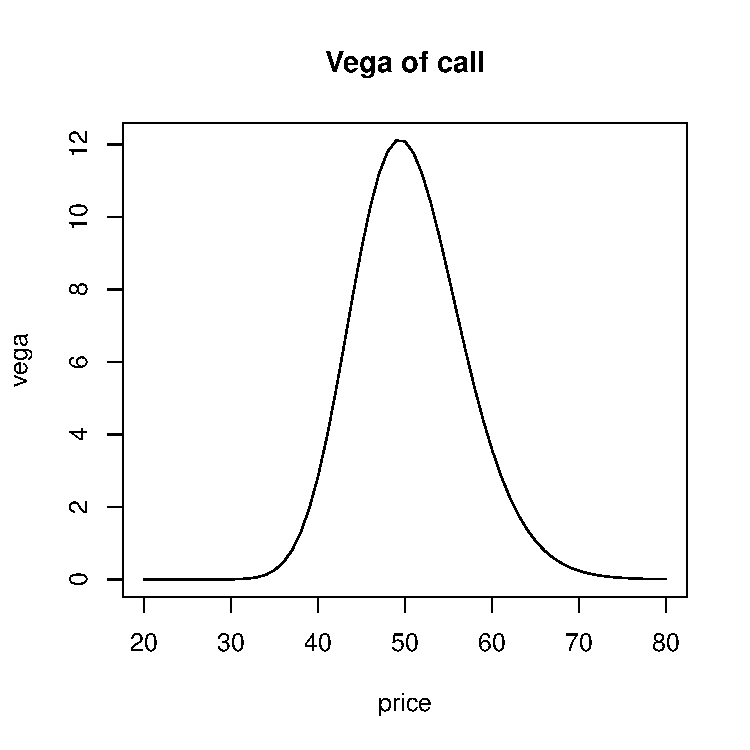
\includegraphics[width=\maxwidth]{figure/unnamed-chunk-19} 

\end{knitrout}


\begin{knitrout}
\definecolor{shadecolor}{rgb}{0.969, 0.969, 0.969}\color{fgcolor}\begin{kframe}
\begin{alltt}
\hlcom{# Vega as the time to maturity varies for in the money, at the money, and}
\hlcom{# out of the money call options}
maturity <- \hlkwd{seq}(0.01, 1, 0.05)
\hlkwd{plot}(maturity, xlim = \hlkwd{range}(maturity), ylim = \hlkwd{c}(0,20), 
     type=\hlstr{"n"}, xlab=\hlstr{"Time to expiration"}, ylab=\hlstr{"Theta"})
\hlkwd{lines}(x = maturity, y = \hlkwd{vegaBS}(55, 50, 0.05, 0, 0.2, maturity, \hlstr{"call"}), 
      lty=2, col=\hlstr{"blue"})
\hlkwd{lines}(x = maturity, y = \hlkwd{vegaBS}(50, 50, 0.05, 0, 0.2, maturity, \hlstr{"call"}), 
      lty=1, col=\hlstr{"black"})
\hlkwd{lines}(x = maturity, y = \hlkwd{vegaBS}(45, 50, 0.05, 0, 0.2, maturity, \hlstr{"call"}), 
      lty=3, col=\hlstr{"red"})
\hlkwd{title}(\hlstr{"Vega of call"})
\hlkwd{legend}(\hlstr{"topleft"}, legend=\hlkwd{c}(\hlstr{"In the money"}, \hlstr{"At the money"}, \hlstr{"Out of the money"}),
       lty=\hlkwd{c}(2,1,3), col=\hlkwd{c}(\hlstr{"blue"}, \hlstr{"black"}, \hlstr{"red"}), bty=\hlstr{"n"}, cex=0.8)
\end{alltt}
\end{kframe}
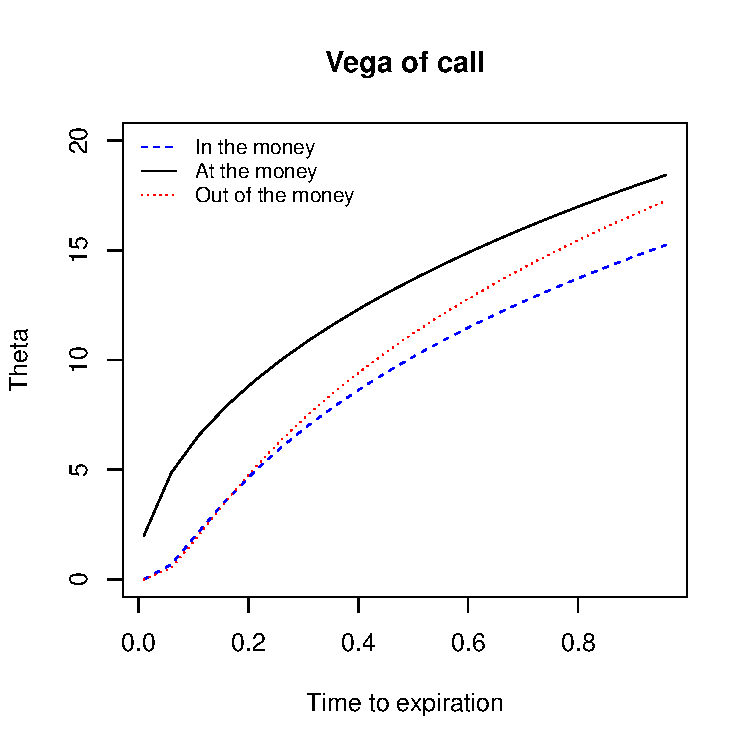
\includegraphics[width=\maxwidth]{figure/unnamed-chunk-20} 

\end{knitrout}


\subsection{Rho}
The rho ($\rho$) of an option is defined as the rate of change of the value of the option with respect to the risk-free interest rate.

The rho of a European option is given as
\begin{eqnarray*}
\rho (call) = K T e^{-r T} N(d_2)\\
\rho (put) = -K T e^{-r T} N(-d_2)\\
\end{eqnarray*}


\begin{knitrout}
\definecolor{shadecolor}{rgb}{0.969, 0.969, 0.969}\color{fgcolor}\begin{kframe}
\begin{alltt}
\hlcom{# Compute the rho of the European call option}
\hlkwd{computeGreeks}(eu.call, \hlstr{"rho"})
\end{alltt}
\begin{verbatim}
## [1] 8.907
\end{verbatim}
\end{kframe}
\end{knitrout}


\begin{knitrout}
\definecolor{shadecolor}{rgb}{0.969, 0.969, 0.969}\color{fgcolor}\begin{kframe}
\begin{alltt}
\hlcom{# Rho as the unerlying price varies}
\hlkwd{computeGreeks}(eu.call, \hlstr{"rho"}, prices = \hlkwd{seq}(20, 80, 1), 
              plot = TRUE, main=\hlstr{"Rho of call"})
\end{alltt}
\end{kframe}
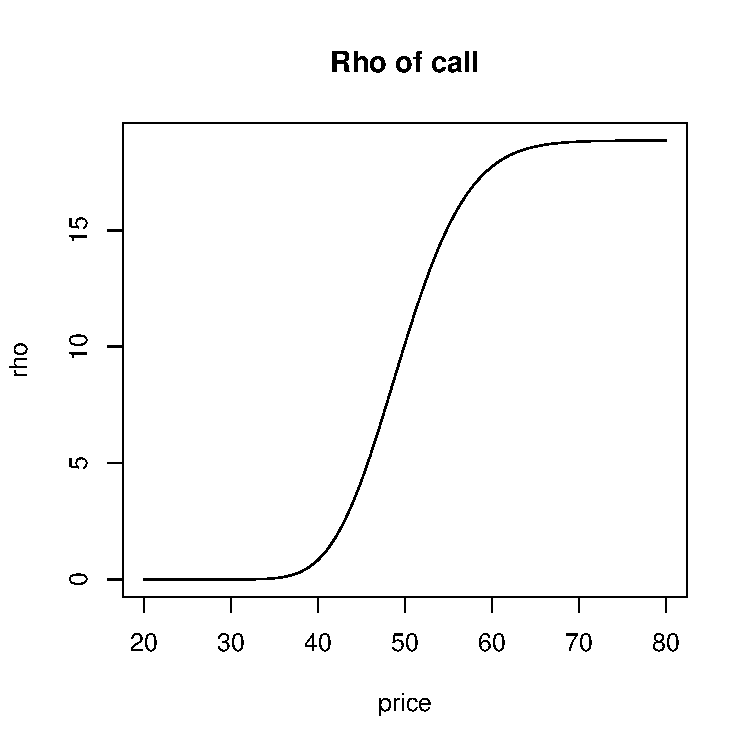
\includegraphics[width=\maxwidth]{figure/unnamed-chunk-22} 

\end{knitrout}


\begin{knitrout}
\definecolor{shadecolor}{rgb}{0.969, 0.969, 0.969}\color{fgcolor}\begin{kframe}
\begin{alltt}
\hlcom{# Rho as the time to maturity varies for in the money, at the money, and}
\hlcom{# out of the money call options}
maturity <- \hlkwd{seq}(0.01, 1, 0.05)
\hlkwd{plot}(maturity, xlim = \hlkwd{range}(maturity), ylim = \hlkwd{c}(0,40), 
     type=\hlstr{"n"}, xlab=\hlstr{"Time to expiration"}, ylab=\hlstr{"Theta"})
\hlkwd{lines}(x = maturity, y = \hlkwd{rhoBS}(55, 50, 0.05, 0, 0.2, maturity, \hlstr{"call"}), 
      lty=2, col=\hlstr{"blue"})
\hlkwd{lines}(x = maturity, y = \hlkwd{rhoBS}(50, 50, 0.05, 0, 0.2, maturity, \hlstr{"call"}), 
      lty=1, col=\hlstr{"black"})
\hlkwd{lines}(x = maturity, y = \hlkwd{rhoBS}(45, 50, 0.05, 0, 0.2, maturity, \hlstr{"call"}), 
      lty=3, col=\hlstr{"red"})
\hlkwd{title}(\hlstr{"Rho of call"})
\hlkwd{legend}(\hlstr{"topleft"}, legend=\hlkwd{c}(\hlstr{"In the money"}, \hlstr{"At the money"}, \hlstr{"Out of the money"}),
       lty=\hlkwd{c}(2,1,3), col=\hlkwd{c}(\hlstr{"blue"}, \hlstr{"black"}, \hlstr{"red"}), bty=\hlstr{"n"}, cex=0.8)
\end{alltt}
\end{kframe}
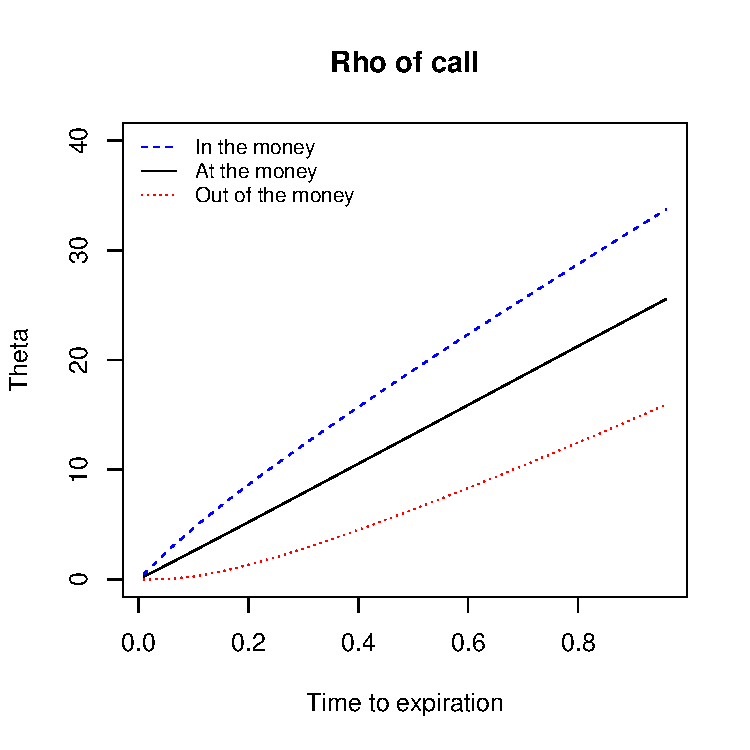
\includegraphics[width=\maxwidth]{figure/unnamed-chunk-23} 

\end{knitrout}


\subsection{Portfolio Insurance}
Example 5.9: A portfolio with worth \$90 million. To protect against market downturns the managers of the portfolio require a 6-month European put option on the portfolio with a strike price of \$87 million. The risk-free rate is 9\% per annum, the dividend yield is 3\% per annum, and the volatility of the portfolio is 20\% per annum. The S\&P 500 index stands at 900. As the portfolio is considered to mimic the S\&P 500 fairly closely, one alternative is to buy 1000 put options on the S\&P 500 with a strike price of 870. Another option is to create the option synthetically. In this case, $S_0 = 90$ million, $K = 87$ million, $r = 0.09$, $q = 0.03$, $\sigma = 0.25$, and $T = 0.5$.

\begin{knitrout}
\definecolor{shadecolor}{rgb}{0.969, 0.969, 0.969}\color{fgcolor}\begin{kframe}
\begin{alltt}
eu.put <- \hlkwd{optionSpec}(style = \hlstr{"european"}, 
                     type = \hlstr{"put"}, 
                     S0 = 90, 
                     K = 87,
                     maturity = 0.5, 
                     r = 0.09,
                     volatility = 0.25,
                     q = 0.03)
\hlkwd{computeGreeks}(eu.put, \hlstr{"delta"})
\end{alltt}
\begin{verbatim}
## [1] -0.3215
\end{verbatim}
\end{kframe}
\end{knitrout}


The delta of the synthetic option is -0.3215. This means that 32.15\% of the portfolio should be sold to match the delta of the synthetic option.

\bibliography{GARPFRM}

\end{document}
